\documentclass{beamer}

\usepackage{natbib}

\usepackage[frenchb]{babel}

\usepackage[T1]{fontenc}

\usepackage[utf8]{inputenc}

\usepackage{amsmath}

\usepackage{tcolorbox}

\usepackage{lipsum}

\usepackage[labelformat=empty]{caption}

\usepackage{cclicenses}

\usetheme{Darmstadt}

\title{Quelle place pour GPG chez Advanced ?}

\author{\cc Ilan 'trog' Dubois}

\AtBeginSection[]
{
    \begin{frame}
        \frametitle{Sommaire}
            \tableofcontents[currentsection]
    \end{frame}
}

\begin{document}
    \begin{frame}
        \titlepage
    \end{frame}
    \section{Mb dszquphsbqijf}
    \subsection{Définitions}
        \begin{frame}{label=vocabulaire}
            \frametitle{Vocabulaire}
            \begin{center}
                \begin{itemize}
                    \item \textbf{Chiffrer}: Rendre incompréhensible un messgae pour qui n'aurait pas la clé.
                    \item \textbf{Déchiffrer}: Rendre à un message sa forme originale à l'aide de la clé.
                    \item \textbf{Décrypter}: Rendre à un message sa forme originale sans utiliser de clé (casser le code).
                    \begin{tcolorbox}[colback=green!5,colframe=green!40!black,title=Mais crypter alors ?]
                      En anglais chiffrer se dit \textit{encrypt}, d'où la confusion courante avec le terme \textit{crypter} qui en français signifie mettre dans une crypte.
                    \end{tcolorbox}
                \end{itemize}
            \end{center}
        \end{frame}
        \begin{frame}{label=utilisation}
            \frametitle{Les cas d'utilisation}
            \begin{center}
                \begin{itemize}
                    \item Rendre incompréhensible un document quelconque pour toute personne n'ayant pas la clé.
                    \item Assurer l'intégrité d'un document.
                    \item Assurer l'authenticité d'un document.
                \end{itemize}
            \end{center}
        \end{frame}
    \subsection{Deux principaux types de cryptographie}
        \begin{frame}{label=symmetric}
            \frametitle{La cryptographie symmétrique}
            \begin{center}
                \begin{itemize}
                    \item Chiffrement et déchiffrement se font avec une même clé.
                    \item César, Vigenaire, AES...
                    \item Est très rapide, utilisé pour chiffrer son disque, sa connexion...
                \end{itemize}
            \end{center}
        \end{frame}
        \begin{frame}{label=asymmetric}
            \frametitle{La cryptographie asymmétrique}
            \begin{center}
                \begin{itemize}
                    \item Utilise une paire de clé \textit{public}/\textit{privé}.
                    \item Le chiffrement se fait avec une clé publique. Le déchiffrement nécessite la clé privée.
                    \item DSA, RSA, Ed25519...
                    \item Plus lent mais aussi très pratique dans le cas où les parties ne partagent pas encore de \textit{secret}. Sert ainsi souvent à initier une connexion avec un chiffrement symmétrique. Votre clé SSH est basé sur ce type de cryptographie.
                \end{itemize}
            \end{center}
        \end{frame}
        \begin{frame}
            \begin{center}
                \begin{figure}
                    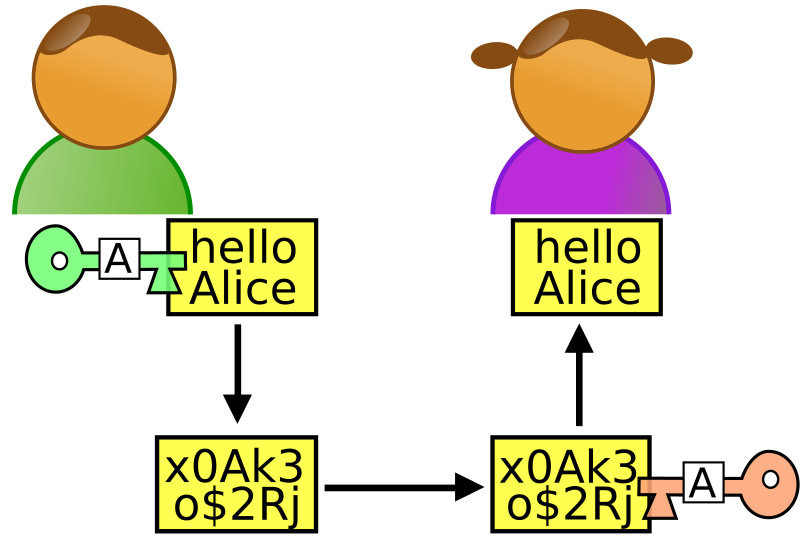
\includegraphics[scale=0.30]{img/asymmetric.png}
                    \caption{\cc --- odder}
                \end{figure}
            \end{center}
        \end{frame}
    \subsection{Bien choisir les paramètres}
        \begin{frame}{label=fails}
            \frametitle{Epic fail}
            \begin{center}
                \begin{figure}
                    
\includegraphics[scale=0.15]{img/plain.jpg}
                    \caption{Image originale}
                \end{figure}
                \pause
                \begin{figure}
                    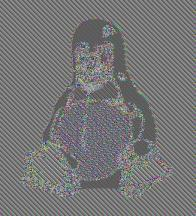
\includegraphics[scale=0.15]{img/aes_no_chain.jpg}
                    \caption{Chiffré sans chaînage}
                \end{figure}
                \pause
                \begin{figure}
                    
\includegraphics[scale=0.15]{img/aes_chain.jpg}
                    \caption{Chiffré avec chaînage}
                \end{figure}
                \cc --- Papa November \& Dr Juzam
            \end{center}
        \end{frame}
    \subsection{Bien choisir les paramètres}
        \begin{frame}{label=playtime}
            \frametitle{Play Time!}
            \begin{center}
                https://github.com/trog-levrai/caesar
                \begin{figure}
                    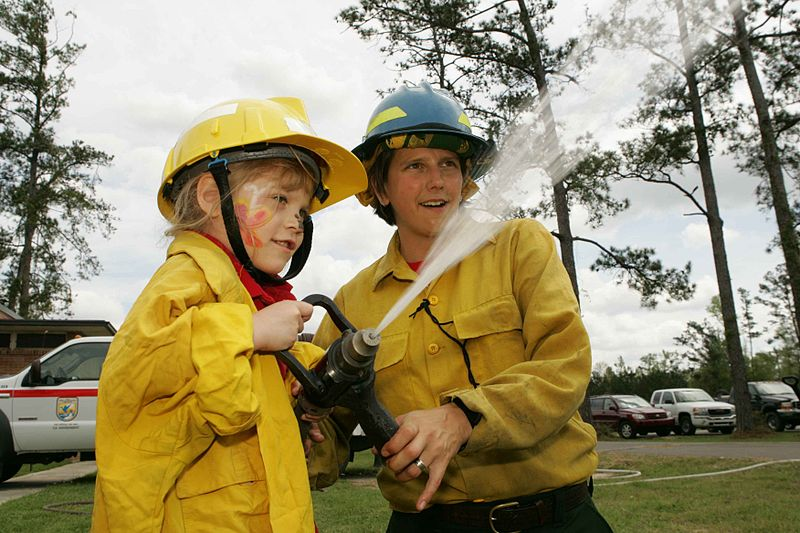
\includegraphics[scale=0.35]{img/playtime.jpg}
                \end{figure}
            \end{center}
        \end{frame}
    \section{PGP}
    \subsection{Présentation}
        \begin{frame}{label=history}
            \frametitle{Un petit historique}
            \begin{center}
                \begin{itemize}
                    \item Protocole inventé en 1991 par Phil Zimmerman, également inventeur de ZRTP.
                    \item L'implémentation la plus connue est GPG (GNU Privacy Guard). Elle est maintenue par un petit groupe, financé depuis peu entre autre par Facebook.
                    \item Sa grande performance et sécurité ont fait que PGP est utilisé pour bien d'autres objectifs aujourd'hui (package manager, versionnement, \ldots)
                    \item Pour contourner la régulation il publia le code sous forme de livre, l'export de livre étant protégé par la constitution américaine. GG
                \end{itemize}
            \end{center}
        \end{frame}
        \begin{frame}{label=utility}
            \frametitle{Utilisation}
            \begin{center}
                \begin{itemize}
                    \item Chiffrer ses communications pour un destinataire \textbf{sans} partage de secret préalable nécessaire.
                    \item \textbf{Authentifier} et assurer l'intégrité des messages par le système de signature.
                    \item Créer un système de confiance \textit{Web of Trust} décentralisé, pas besoin de signature d'une autorité externe.
                    \item Git supporte très bien l'utilisation de GPG, je vous recommande de signer au moins vos tags, ce qui permettra d'authentifier les versions qui seront utilisées.
                \end{itemize}
                \begin{tcolorbox}[colback=green!5,colframe=green!40!black,title=Pourquoi authentifier ?]
                    La signature permet d'authentifier l'origin d'un fichier. On peut donc s'assurer qu'un build, une release ou autre n'a pas été modifié.
                    Dans le cas d'un programme, on s'assure alors qu'aucune back door n'a été ajoutée par exemple ;)
                \end{tcolorbox}
            \end{center}
        \end{frame}
        \begin{frame}{label=keychain}
            \frametitle{Keychain}
            La \textbf{keychain} est l'ensemble des clés connues de GPG.
            \begin{center}
                \begin{itemize}
                    \item Stocke les clés publiques de vos contacts ainsi que toutes les informations associées.
                    \item Stocke vos paires de clé publique/privé.
                    \item Il est très facile de télécharger de nouvelles clés depuis les différents serveurs de clé.
                \end{itemize}
                \begin{tcolorbox}[colback=green!5,colframe=green!40!black,title=Pour mettre à jour la keyring]
                    > gpg -{}-refresh-keys
                \end{tcolorbox}
            \end{center}
        \end{frame}
        \begin{frame}
            \frametitle{Man in the middle}
            \begin{center}
                \begin{figure}
                    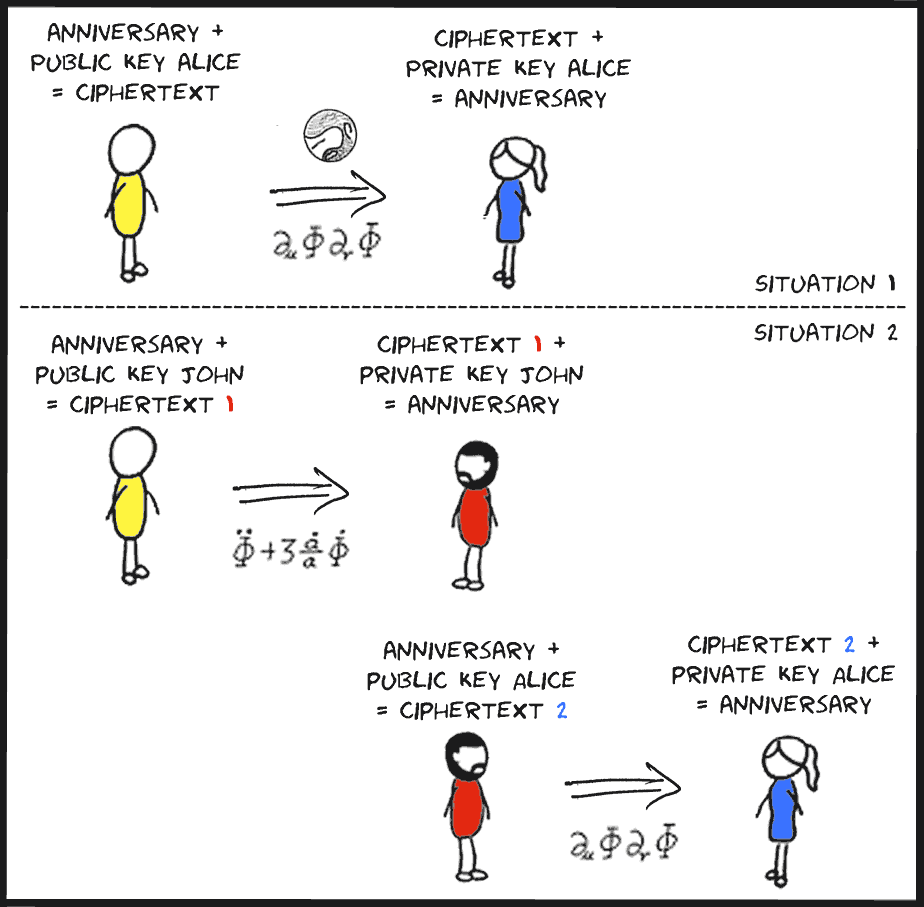
\includegraphics[scale=0.2]{img/mitm.png}
                    \caption{\cc --- Abstruse Goose}
                \end{figure}
            \end{center}
        \end{frame}
        \begin{frame}{label=trust}
            \frametitle{Web of Trust}
            \textbf{Web of Trust} est le concept utilisé par PGP pour assurer que les clés sont bien détenues par leur propriétaire déclaré.
            \begin{center}
                \begin{itemize}
                    \item Chaque clé peut signer ou être signée par une autre clé. Différents degré de confiance est accordé à chaque signature.
                    \item La possibilité pour tout le monde de signer des clés évite d'avoir à \textit{croire} une autorité unique et externe.
                    \item La toile de confiance ainsi crée vous permet de récupérer des clés de façon fiable.
                    \item Les clés et leur signatures doivent être disponibles sur un serveur de clés pour propager les clés et leur signature.
                    \item Avec une clé Advanced Schema et des signatures multiples entre détenteurs de clé, la toile de confiance est largement suffisante.
                \end{itemize}
            \end{center}
        \end{frame}
        \begin{frame}
            \frametitle{Exemple de Web of Trust}
            \begin{center}
                \begin{figure}
                    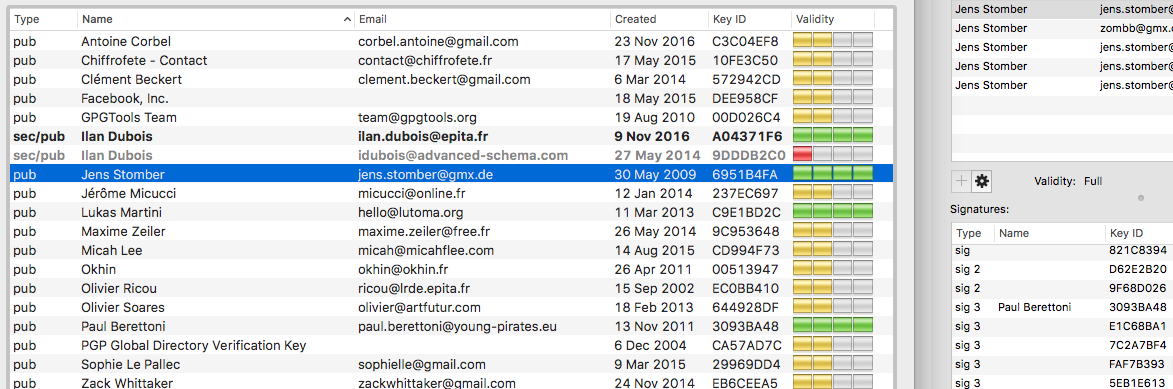
\includegraphics[scale=0.27]{img/trust.png}
                \end{figure}
            \end{center}
        \end{frame}
        \begin{frame}{label=signin}
            \frametitle{Pourquoi signer ?}
            Une \textbf{signature cryptographique} est le procédé qui permet d'assurer que le détenteur de la clé de signature en approuve le contenu.
            \begin{center}
                \begin{itemize}
                    \item GPG support très bien l'utilisation de ce procédé et permet aisin de vérifier l'origine des documents signés.
                    \item Cela permet d'éviter qu'un attaquant ne puisse modifier le message envoyé.
                    \item Pour du code ou un binaire, cela évite les back-doors par exemple.
                    \item Le système de signature est très fiable, il s'agit simplement du système de chiffrement inversé.
                    \item C'est pourquoi GPG va vous générer des sous-clés \textbf{SC} (signe et certifie) et \textbf{E} (chiffre).
                \end{itemize}
            \end{center}
        \end{frame}
        \begin{frame}
            \begin{center}
                \begin{figure}
                    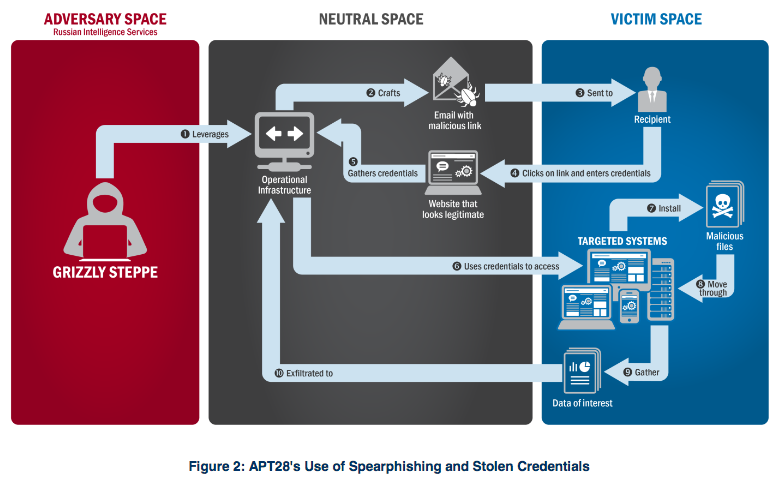
\includegraphics[scale=0.35]{img/signature.png}
                    \caption{Attaque du collège éléctoral américain pour l'éléction 2016}
                \end{figure}
            \end{center}
        \end{frame}
    \subsection{Mise en route}
        \begin{frame}{label=generate}
            \frametitle{Installation}
            Pour la gestin des clés, une installation suffira \cite{best}:
            \begin{center}
                \begin{itemize}
                    \item GNU/Linux: rien à faire
                    \item Windows: installer Gpg4win
                    \item MacOS: installer GPG Suite from GPG Tools (pas nécessaire mais pratique)
                \end{itemize}
            \end{center}
            \begin{tcolorbox}[colback=green!5,colframe=green!40!black,title=Configuration]
                Pour augmanter encore un peu la robustesse, je vous conseil d'utiliser la configuration duraconf pour GPG.
                Vous pourrez remplacer keyserver et ses options pour le serveur de clés Advanced.
                Une fois la clé génrérée, remplacer default-key
            \end{tcolorbox}
        \end{frame}
        \begin{frame}
            \begin{center}
                \begin{figure}
                    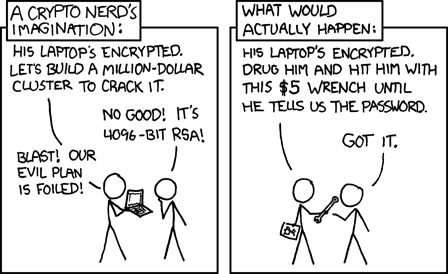
\includegraphics[scale=0.60]{img/security.png}
                    \caption{\cc --- xkcd}
                \end{figure}
            \end{center}
        \end{frame}
        \begin{frame}{label=email}
            \frametitle{Client mail}
            Un client mail adapté sera nécessaire pour chiffrer et signer ses mails
            \begin{center}
                \begin{itemize}
                    \item Thunderbird + Enigmail
                    \item Outlook + GpgpOl (intallé avec Gpg4win)
                    \item Mail + GPGMail (pas encore pour Sierra)
                    \item K9Mail + APG pour Android
                \end{itemize}
            \end{center}
        \end{frame}
        \begin{frame}{label=generate}
            \frametitle{Génération des clés}
            Ouvrez l'option de génération de votre outil favoris et utilisez les paramètres suivants:
            \begin{center}
                \begin{figure}
                    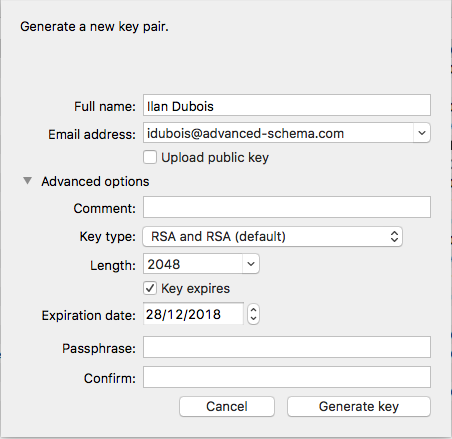
\includegraphics[scale=0.40]{img/gen.png}
                \end{figure}
            \end{center}
        \end{frame}
        \begin{frame}{label=revoke}
            \frametitle{Certificat de révocation}
            Si vous perdez accès à votre clé privée, ou que celle-ci est compromise, vous pouvez le faire savoir à l'aide du certificat de révocation.
            Celui-ci indique que pour une raison ou pour une autre, il ne faut plus utiliser cette clé. Il est donc important que vous le génériez et que vous en gardiez une copie (chiffrée symmétriquement).
        \end{frame}
        \appendix
        \begin{frame}
            \bibliography{src/crypto}{}
            \bibliographystyle{plain}
        \end{frame}
\end{document}
